\section{Source-specific proof of the delivered mission}\label{sec:proof}
\subsection{A weight that remains valid under rate uncertainty}
Use
\begin{equation}\label{eq:w}
 w=(14,11,10,84,43,107)^\top,\qquad w_{\min}=10.
\end{equation}
Direct rational evaluation of~\eqref{eq:A} at the endpoints gives
\begin{align}\label{eq:nominal}
 A_ew&\le-\frac{99}{1000}w &&(29/100\le e\le31/100),\nonumber\\
 A_ew&\le\frac{67}{500}w &&(1/100\le e\le31/100).
\end{align}
The endpoint checks suffice because each component of $A_ew/w$ is affine in $e$, so its maximum over an interval is attained at an endpoint. The reconstructed row values and their checked inequalities are given in Appendix~\ref{app:certificates}. In particular the largest weighted drift ratios at $e=.01,.29,.31$ are, respectively,
\[
 \frac{559}{4200},\qquad-\frac{533}{5350},\qquad-\frac{73}{700}.
\]

If $\widetilde A_e$ belongs to the one-percent box of Remark~\ref{rem:box}, then changing off-diagonal chemistry rates also changes their diagonal row sums. Accounting for both changes gives, for each type,
\begin{align}\label{eq:error}
 |((\widetilde A_e-A_e)w)_i|
 &\le\frac1{100}\left[
 \sum_{j\ne i}(Q_e)_{ij}|w_j-w_i|
 +\frac1{10}\,|(Lw)_i-w_i|+d_iw_i\right]\nonumber\\
 &\le\frac{27}{2000}\,w_i,\qquad 1/100\le e\le31/100.
\end{align}
The three terms are the chemistry, division and mortality contributions. The bracket divided by $w_i$ is affine and nondecreasing in $e$, so it is maximal at $e=31/100$, where its largest value is $1427/1075<27/20$. The envelope therefore covers every point of the box, not a sample of perturbed models. From~\eqref{eq:nominal}--\eqref{eq:error},
\begin{equation}\label{eq:robustdrift}
 \widetilde A_ew\le g\,w\quad\hbox{on }[.01,.31],\qquad
 \widetilde A_ew\le-\gamma\,w\quad\hbox{on }[.29,.31],\qquad
 g=\frac{59}{400},\quad\gamma=\frac{171}{2000}.
\end{equation}

\subsection{Delivery, extinction and the healthy path}
\begin{proof}[Proof of Theorem~\ref{thm:main}]
For the fixed course~\eqref{eq:course}, concentration is
\begin{equation}\label{eq:concentration}
 c(t)=\begin{cases}
 \dfrac{29}{100k_e}(1-e^{-k_et}),&0\le t\le112,\\[4pt]
 c(112)e^{-k_e(t-112)},&112<t\le120.
 \end{cases}
\end{equation}
Consequently $0\le c(t)\le29/99<3/10$ uniformly. For $4\le t\le112$, bounding $1/k_e$ and $1-e^{-k_et}$ separately from below,
\begin{equation}\label{eq:band}
 c(t)\ge\frac{29}{101}\left(1-e^{-99/25}\right)
 >\frac{29}{101}\cdot\frac{49}{50}=\frac{1421}{5050}>\frac{28}{100},
\end{equation}
where $e^{99/25}>50$ follows from a positive Taylor sum through degree~$15$. Hence the effective erasure $e=1/100+c$ lies in $[.01,.31]$ throughout and in $[.29,.31]$ on $[4,112]$: the first four units lie in the growth interval of~\eqref{eq:robustdrift} and the next $108$ units lie in its contraction interval.

For $Y_t=Z_t\cdot w$, localization at target count $N$ together with the generator identity yields the corresponding expectation inequalities; the Yule domination of Section~\ref{sec:model} provides the integrable finite-horizon bound needed to let $N\to\infty$. Gronwall's inequality and $Y_t\ge w_{\min}\1_{\{|Z_t|>0\}}$ then give
\begin{align}\label{eq:targetproof}
 \Prob(|Z_{112}|>0)
 &\le\frac{4\cdot107}{10}\exp(4g-108\gamma)\nonumber\\
 &=\frac{214}{5}\exp\left(-\frac{2161}{250}\right)
 <\frac{214/5}{5000}=\frac{107}{12500}.
\end{align}
Indeed $2161/250>43/5$, and the positive Taylor sum for $e^{43/5}$ through degree~$30$ exceeds $5000$. No target immigration is present, so extinction is absorbing and survival at $120$ implies survival at $112$; it is unnecessary to assume contraction during washout.

For healthy units,~\eqref{eq:box} and the uniform concentration bound imply
\begin{equation}\label{eq:healthym}
 m_H(t)\le\frac{3/10+29/99}{2}+\frac1{200}<\frac{61}{200}=:m .
\end{equation}
Apply Theorem~\ref{thm:anchor} with $K=400$, $h_{\min}=200$, $M=278$, $\reff=1$, $m=61/200$ and the full horizon $T=120$. Its simpler product bound is
\begin{equation}\label{eq:certificate}
 278\cdot\frac{61}{200}\cdot120
 \prod_{h=200}^{277}\frac{122}{400-h}
 <\frac7{10^6},
\end{equation}
an exact rational inequality. Every initial count allowed by~\eqref{eq:box} is at least the anchor. The bound counts crossings followed by later recovery, and it already includes the entire washout period. Combining it with~\eqref{eq:targetproof} proves the two marginal statements in~\eqref{eq:mainbounds} and, by the union bound,~\eqref{eq:joint}.

Finally, the total administered amount is $112(29/100)=812/25=32.48<33$. Integrating~\eqref{eq:pk} gives
\begin{equation}\label{eq:amount}
 k_e\int_0^{120}c(t)\,dt
 =\int_0^{120}a(t)\,dt-c(120),\qquad
 \int_0^{120}c(t)\,dt\le\frac{3248}{99}<33.
\end{equation}
The amplitude limits $a\le3/10$ and $c\le29/99<3/10$ have already been checked. The post-stop concentration integral is at most $2900/9801$ and was not removed from the healthy law. Every step holds for all parameters in~\eqref{eq:box} and all target-rate factors in the declared box under the same fixed administration. This proves the theorem.
\end{proof}

\begin{figure}[tb]
 \centering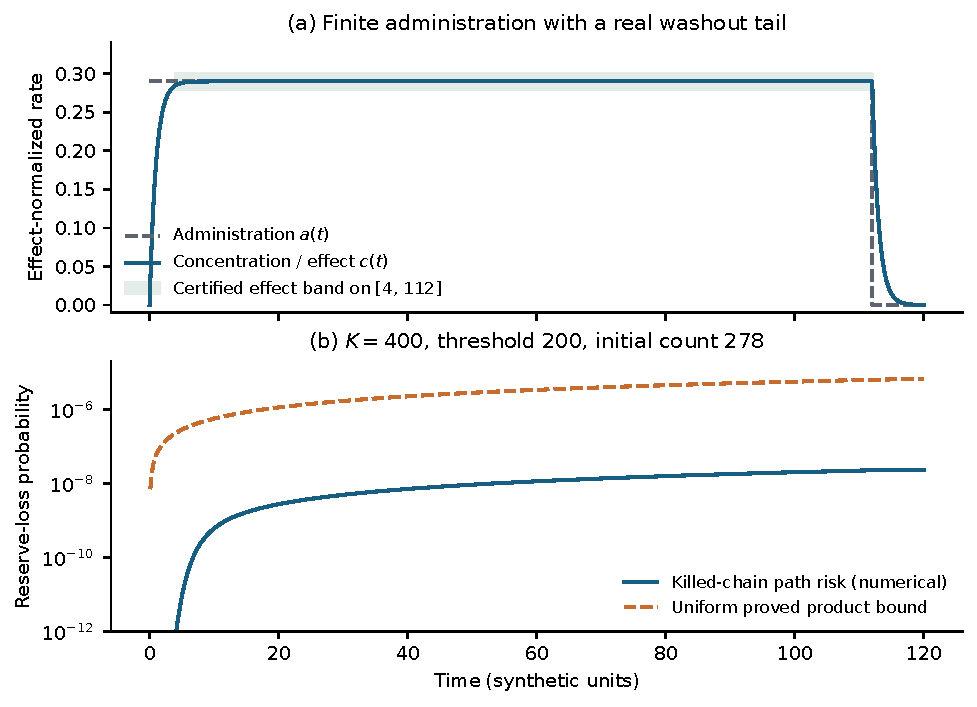
\includegraphics[width=.94\linewidth]{figures/delivered_course.pdf}
 \caption{The delivered course and reserve risk. The concentration curve uses nominal clearance $k_e=1$; the band and probability envelope are uniform over the theorem's box. The healthy curve solves the killed forward equation numerically at $K=400$, $h_{\min}=200$, $H_0=278$, $\reff=1$, $\sigma=2$, $\nu=.005$ for that one parameter trajectory. It is an illustrative floating computation, not a Monte Carlo estimate and not the certificate. The dashed bound uses the worst constant mortality, is uniform over the box, and retains all threshold crossings; the two curves are therefore different probabilistic objects, which is why the visible gap is not a measure of looseness at a fixed parameter.}\label{fig:course}
\end{figure}

The proof uses only three properties of the input: an effective-erasure band, a healthy mortality ceiling, and the administration constraints. For other response laws, including saturating ones, the same implication holds whenever the actual delivered trajectory satisfies those three requirements. Such a statement is conditional on a checked response band; it is not evidence that an arbitrary Hill law realizes this example, and if saturation prevents entry into the band then this weight certifies nothing about that course either way.

\subsection{How little reserve the same course needs}\label{sec:cheap}
The hypotheses on $H_0$ and $K$ in~\eqref{eq:box} were chosen to make the healthy margin comfortable, not to make the mission feasible. Two exact-arithmetic consequences quantify the difference. Both keep the administration~\eqref{eq:course}, the target uncertainty box, the four $AA$ founders, $T=120$, $\reff\ge1$, $\sigma\in[2,3]$, $\nu\in[0,1/200]$ and $k_e\in[.99,1.01]$; hence the target bound~\eqref{eq:targetproof} is unchanged and only the healthy side moves.

\begin{corollary}[Mission tolerance survives a nearly depleted reserve]\label{cor:filling}
In the setting of Theorem~\ref{thm:main} with $K=400$ and $h_{\min}=200$, replace the requirement $H_0\ge278$ by $H_0\ge h_0$. Then, evaluating~\eqref{eq:initial} with $M=278$ in exact rational arithmetic,
\[
 \Prob(\tau_H\le120)<
 \begin{cases}
 9.827\times10^{-3},& h_0=209,\\
 8.191\times10^{-5},& h_0=221,\\
 2.908\times10^{-6},& h_0=240 .
 \end{cases}
\]
In particular both mission tolerances $\delta=\alpha=1/100$ are met from any initial count $h_0\ge209$, with joint success greater than $0.98161$; and $h_0\ge240$ gives joint success greater than $0.991437$. The value $209$ is the exact minimum for which this certificate meets $\alpha=1/100$: at $h_0=208$ the same expression exceeds $1/100$.
\end{corollary}

\begin{proof}
The right-hand side of~\eqref{eq:initial} is nonincreasing in $h_0$ by Corollary~\ref{cor:initial}, so it suffices to evaluate it at the displayed counts. With $K=400$, $h_{\min}=200$, $M=278$, $\reff=1$, $m=61/200$, $T=120$ one has $D_{278}=2.5980909040\ldots$ and $MmTq_M=2.6704763715\ldots\times10^{-6}$, and the initial scale term $\sum_{j\ge h_0}P_j/D_M$ evaluates to $9.8243\times10^{-3}$, $7.9238\times10^{-5}$ and $2.3748\times10^{-7}$ at $h_0=209,221,240$. Adding the two terms gives the displayed bounds. The target bound~\eqref{eq:targetproof} is unaffected, and the union bound gives the joint statements. All quantities are ratios of integers and were evaluated exactly.
\end{proof}

\begin{corollary}[A smaller sufficient reserve at the same tolerances]\label{cor:smaller}
Keep every assumption of Theorem~\ref{thm:main} except the reserve preparation, and take instead
\[
 K=232,\qquad h_{\min}=116,\qquad M=161,\qquad H_0\ge161 .
\]
Then $\Prob(\tau_H\le120)<9.781\times10^{-3}<1/100$ and $\Prob(|Z_{120}|>0)<107/12500$, so both mission tolerances hold and
\[
 \Prob(Z_{120}=0,\ \tau_H>120)>0.98165 .
\]
\end{corollary}

\begin{proof}
The threshold is again half of capacity and the anchor is again the worst-case equilibrium count, $\lfloor232(1-.305)\rfloor=161$. With $\reff=1$, $m=61/200$ and $T=120$, the first bound of~\eqref{eq:anchorbound} gives
\[
 \Prob(\tau_H\le120)\le\frac{MmT\,P_{M-1}}{D_M}
 =\frac{161\cdot\frac{61}{200}\cdot120}{D_{161}}
 \prod_{h=116}^{160}\frac{232\cdot\frac{61}{200}}{232-h}
 =9.7801\ldots\times10^{-3},
\]
with $D_{161}=2.6271217\ldots$, again an exact rational quantity. The mortality ceiling~\eqref{eq:healthym} and the target argument are untouched by the change of reserve, so~\eqref{eq:targetproof} still applies and the union bound gives the joint statement.
\end{proof}

\begin{remark}[The denominator is doing real work here]\label{rem:cruder}
Corollary~\ref{cor:smaller} uses the sharper of the two bounds in~\eqref{eq:anchorbound}. The cruder product $MmTP_{M-1}$ alone equals $2.569\times10^{-2}$ at $K=232$ and does not meet the tolerance; the smallest capacity it certifies in this proportional family is $K=252$, where it gives $9.831\times10^{-3}$. Within the same family, $K=232$ is the smallest capacity certified by the sharper bound. Neither statement is a minimum-capacity theorem: both are sufficient constructions from one proof method, and no converse excludes smaller reserves.
\end{remark}
